%-------------------------- model.tex -------------------------%
%Exemple per a usar l'estil tfm.class per a la preparaci\'o
%de monografies de treballs final de m\`aster.
%
%
%----------------------------- FMETFM ----------------------------%
\documentclass[reqno,twoside, 12pt]{report}

\usepackage[spanish,english]{babel}
\usepackage[table,xcdraw]{xcolor}
\usepackage{pdfpages}
\usepackage[thinlines]{easytable}
\usepackage[utf8]{inputenc}
\usepackage{amsmath}
\usepackage{hyperref}
\usepackage{mathtools}
\usepackage{hyperref}
\usepackage{graphicx}
\usepackage{algorithm}
\usepackage{algpseudocode}
\usepackage{parskip}
\usepackage{xcolor,colortbl}
\usepackage{fancyhdr}
\usepackage[export]{adjustbox}
\usepackage{rotating}
\usepackage{wrapfig}
\usepackage{epstopdf}
\usepackage{float}
\usepackage{eurosym} 
\usepackage{subcaption}
\usepackage{lscape}
\usepackage{lipsum}
\usepackage{amsfonts}
\usepackage{tikz}
\usetikzlibrary{matrix,chains,positioning,decorations.pathreplacing,arrows}

%Para introducir trozos de código
\usepackage{listings}
\lstloadlanguages{R}
\lstset{language=R,
	basicstyle=\small\ttfamily,
	stringstyle=\color{dkgreen},
	otherkeywords={0,1,2,3,4,5,6,7,8,9},
	morekeywords={TRUE,FALSE},
	deletekeywords={\_},
	keywordstyle=\color{blue},
	commentstyle=\color{DarkGreen},
}


\usepackage{color}
\definecolor{gray97}{gray}{.97}
\definecolor{mauve}{rgb}{0.58,0,0.82}
\definecolor{dkgreen}{rgb}{0,0.6,0}
\definecolor{greentable}{rgb}{0.176, 0.682, 0.396}

%hasta aquí
\usepackage{caption} 
\usepackage{pdflscape}
\usepackage{appendix}
\definecolor{blue}{rgb}{0.372, 0.847, 0.835}
\usepackage[table]{xcolor}
\newcommand{\specialcell}[2][c]{%
	\begin{tabular}[#1]{@{}l@{}}#2\end{tabular}}

\newtheorem{definition}{Definition}[chapter]

\pagestyle{fancy}
\fancyhf{}
\fancyhead[LE,RO]{}
\fancyhead[RE,LO]{\rightmark}
\fancyfoot[CE,CO]{\thepage}
\fancyfoot[LE,RO]{}

\renewcommand{\headrulewidth}{2pt}
\renewcommand{\footrulewidth}{1pt}

\newcolumntype{L}[1]{>{\raggedright\let\newline\\\arraybackslash\hspace{0pt}}m{#1}}
\newcolumntype{C}[1]{>{\centering\let\newline\\\arraybackslash\hspace{0pt}}m{#1}}
\newcolumntype{R}[1]{>{\raggedleft\let\newline\\\arraybackslash\hspace{0pt}}m{#1}}

\setcounter{tocdepth}{5}

%%-------------------------------------------------------------%
\begin{document}

% Seleccioneu l'idioma:
%\selectlanguage{catalan}
\selectlanguage{spanish}
%\selectlanguage{english}

%----------------------------------------------------------------
% Inici del document
%------------------------------------------------------------------
\begin{titlepage}
 
\newlength{\centeroffset}
\setlength{\centeroffset}{-0.5\oddsidemargin}
\addtolength{\centeroffset}{0.5\evensidemargin}
\thispagestyle{empty}

\noindent\hspace*{\centeroffset}\begin{minipage}{\textwidth}

\centering

\includegraphics[width=0.6\textwidth]{imagenes/logo_ugr.jpg}\\[1.4cm]

\textsc{ \Large TRABAJO FIN DE GRADO\\[0.2cm]}
\textsc{ DOBLE GRADO EN INGENIERÍA INFORMÁTICA Y MATEMÁTICAS}\\[1cm]
% Upper part of the page
% 
% Title
{\Huge\bfseries Análisis de sentimientos \\
}
\noindent\rule[-1ex]{\textwidth}{3pt}\\[3.5ex]
{\large\bfseries Aplicación de Deep Learning para la extrancción de características.}
\end{minipage}

\vspace{0.1cm}
\noindent\hspace*{\centeroffset}\begin{minipage}{\textwidth}
\centering

\textbf{Autor}\\ {Nuria Rodríguez Barroso}\\[2.5ex]
\textbf{Directores}\\
{Francisco Herrera Triguero\\
Mª Victoria Luzón García}\\[2cm]

\includegraphics[width=0.3\textwidth]{imagenes/etsiit_logo.png}\\[0.1cm]
\textsc{Escuela Técnica Superior de Ingenierías Informática y de Telecomunicación}\\
\textsc{---}\\
Granada, septiembre de 2018
\end{minipage}
%\addtolength{\textwidth}{\centeroffset}
%\vspace{\stretch{2}}
\end{titlepage}




%-----------------------------------------------------------------
% P�gina inicial
%-----------------------------------------------------------------
%\title{Sentiment Analysis For Touristic Attractions: \\
%A Case Study On The Alhambra}
%
%\def\autor{Ana Valdivia Garc\'{\i}a}
%
%\def\treball{Mater's degree thesis}
%
%
%\def\advisor{Salvador Garc\'{\i}a L\'{\o}pez}
%
%
%
%\vfill
%
%\def\departament{Computer Science and Artificial Intelligence}
%

%-------------------------------------------------------------%
%\maketitle

%-------------------------------------------------------------%
%%%Dedicatoria (opcional)
%-------------------------------------------------------------%
% \cleardoublepage
%\includepdf[pages={1-}]{Dedicatoria.pdf}
%\cleardoublepage
%%-------------------------------------------------------------%
%%-------------------------------------------------------------%
%%%%Prefaci (opcional)
%%-------------------------------------------------------------%
%%----------------------------------------------------------------
%% Declaraci� d'originalitat
%%------------------------------------------------------------------
%\includepdf{DeclaracionOrginalidad.pdf}
%\cleardoublepage
%%-----------------------------------------------------------------
%
%
%%\begin{comment}
%%\begin{preface}
%%\thispagestyle{empty}
%% Tot i que no �s obligat�ria la seva pres�ncia,
%%el pr�leg i el prefaci s�n dos apartats que normalment apareixen a
%%les obres. La funci� de tots dos �s transmetre opinions o reflexions
%%sobre l'obra, explicar el proc�s d'elaboraci� o argumentar-ne
%%l'oportunitat. El pr�leg el redacta una persona diferent de l'autor,
%%i el prefaci, l'autor mateix.
%%\end{preface}
%%\cleardoublepage
%%\end{comment}
%
%%---------------------------------------------------------------
%% Abstract: un resum del contingut del treball (sobre 500 paraules)
%% Ha de contenir una relaci� de paraules clau i dels codis MSC
%%(Math. Subject Classification 2000)
%% Ha d'estar tamb� en angl�s.
%%---------------------------------------------------------------
%%
\includepdf[pages={1}]{pagina_en_blanc.pdf}
%
%\pagenumbering{roman} \setcounter{page}{7} \markboth{}{}
%
%\begin{abstract}
%The development of Web 2.0 has led to an important amount of content in webpage. Users are free to express their opinions about products, places and events. This project research is aimed at introducing sentiment analysis into touristic attractions. To begin with, we scrap TripAdvisor reviews from the most touristic attraction in Spain, the Alhambra. We then create two sentiment labels: the expert sentiment which is the rate of the reviewer; and the machine sentiment which is extracted from a Natural Language Processing toolkit developed in Stanford University. After that, we build classification models so as to predict polarity sentiments. Finally, we develop a subgroup discovery method so as to extract valuable information about negative reviews.
%
%\vspace{1cm}
%
%\textbf{Key words:} opinion mining, sentiment analysis, tourism, natural language processing, subgroup discovery
%\end{abstract}
%
%%\cleardoublepage
%
%%%%%%%%%%%%%%%%%%%%%%%%%%%%%%%%%%%%%%%%%%%%%%%%%%%%%%%%%%%
%%%Notation (optional)
%%%%%%%%%%%%%%%%%%%%%%%%%%%%%%%%%%%%%%%%%%%%%%%%%%%%%%%%%%%
%%\begin{notation}
%%\begin{tabular}{cl}
%%$(a,b)$ & The greatest common divisor of $a$ and $b$\\[0.3em]
%%$\parity{P}{Q}$  & Number of prime factors of $Q$, taken positively and counted with multipicity,\\[0.3em] & such that $P$ is nonresidue of them.\\[0.3em]
%
%%${\mathbb Z}$ & Nombres enters\\[0.3em]
%%${\mathbb Q}$ & Nombres racionals\\[0.3em]
%%${\mathbb R}$ & Nombres reals\\[0.3em]
%%${\mathbb C}$ & Nombres complexos
%%\end{tabular}
%%\end{notation}

%--------------------------------------------------------------
% Taula de continguts
% S'elabora autom�ticament
%-------------------------------------------------------------

\pagenumbering{roman}
\pagestyle{plain}

\setcounter{page}{10}

\includepdf[pages={1-}]{primeraspaginas}
\pagenumbering{gobble}
\tableofcontents

\clearpage

%------------------------------------------------------------
% Cos del treball
%Es poden fer servir Parts, Capitols, Seccions i Subseccions
%-------------------------------------------------------------
\pagenumbering{arabic}
\pagestyle{fancy}
\renewcommand{\thesection}{\arabic{chapter}.\arabic{section}}
\setcounter{page}{11}

\chapter{Introducción} \label{intro}
	
	\section{Contexto} \label{context}
	
	%	TESIS EUGENIO:
	%	Desarrollar aqui el comportamiento humano -> pedir / hacer opiniones
	%	Evolución histórica de la opinión -> Hasta web 2.0
	
	La principal característica del ser humano y la que le diferencia del resto de seres vivos es la racionalidad. El ser humano utiliza la razón para la toma de decisiones, contemplando los diferentes escenarios y evaluando la mejor manera de alcanzar sus objetivos. Sin embargo, el ser humano consta de una racionalidad limitada, por lo que el abanico de posibilidades que baraja en cada momento está limitado por su visión de la realidad. 
	
	Es por esto que el proceso de toma de decisiones constituye un gran reto. Para facilitar el proceso de toma de decisiones y con el fin de ampliar el abanico de consecuencias contempladas, es muy común la acción de ``pedir opinión'' a terceros.
	
	 La ayuda en la toma de decisiones no es la única función de las opiniones. Las personas también utilizamos las opiniones para expresar nuestro juicio acerca de variados temas. Cuando se produce un intercambio de opiniones ambos participantes se enriquecen con el punto de vista del contrario. 
	 
	El uso de las opiniones ha evolucionado con el ser humano a lo largo de la historia. Comenzando en los inicios del lenguaje, pasando a estar por escrito con la llegada de la escritura y disparándose con el auge de la difusión de opinión en la prensa con la invención del a imprenta.
	
	Uno de los acontecimientos más influyentes en la sociedad fue la invención de Internet en la segunda mitad del s. XX. Trajo consigo una gran fuente de información de fácil acceso. A principios del s.XXI enfatizó el cambio social que ya estaba ocurriendo un nuevo concepto de Web, la Web 2.0. Este innovador concepto ofrecía a todo usuario de ella la posibilidad de compartir todo tipo de información en Internet. Así fue como se preparó el camino para la llegada de las redes sociales, los blogs, o los foros. Plataformas donde los usuarios podían compartir todo tipo de pensamientos u opiniones sin ningún flitro. También se sumaron al carro de la Web 2.0 las empresas. Muchas de ellas incorporaron la opción de compra \textit{online} suponiendo una nueva fuente de ingresos e incluso surgieron muchas nuevas empresas que llevan a cabo toda su funcionalidad a través de Internet.
	
	%Poner aquí una frase final que no se quede como en el aire 

	
	\section{Motivación} \label{motivacion}
	%	TFG MIGUEL:
	%	Conectando con lo anterior -> hay muchísimas opiniones en internet
	%	Aparición de grandes empresas
	%	Las empresas quieren/necesitan conocer la opinión/éxito/fracaso de sus productos 
	%	para los procesos de marketing y para posibles mejoras

	En el contexto de la Sección \ref{context}, tanto el auge de las redes sociales como la incorporación de las empresas al negocio \textit{online} no trajeron consigo solo nuevas fuentes de beneficios. La Web 2.0 supuso una nueva (y enorme) fuente de información. Esta generación exponencial de datos de naturaleza desestructurada en Internet propició el nacimiento de lo que hoy conocemos como \textit{Big Data}.
	
	\begin{figure}[h!]
		\centering
		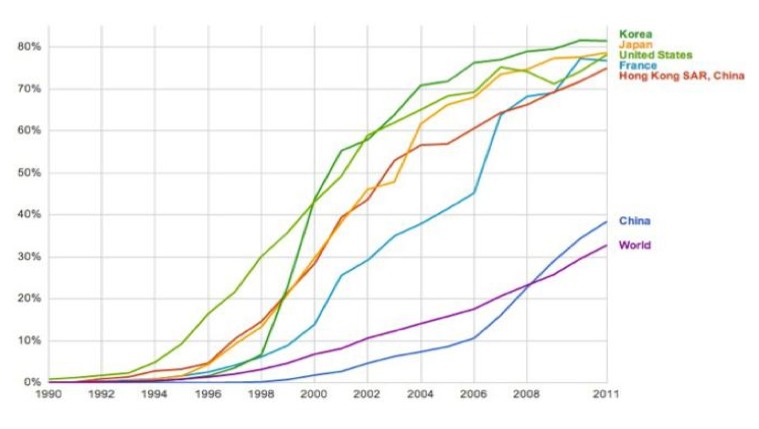
\includegraphics[width=0.7\linewidth]{imagenes/grafica-intro}
		\caption{Gráfica del crecimiento del \textit{Big Data} en algunos países y en el mundo.}
		\label{fig:grafica-intro}
	\end{figure}
	 
	 Para hacernos una idea del impacto del nacimiento de la Web 2.0, observamos la Figura \ref{fig:grafica-intro} en la que se representa el crecimiento de \textit{Big Data} en algunos países desarrollados y en el mundo en general. Notamos que en el año 1998 se produce un aumento en el ritmo de crecimiento, coincidiendo con el nacimiento de la Web 2.0. El siguiente cambio de crecimiento más brusco lo encontramos en el año 2006, año de mayor impacto de las redes sociales. 
	 
	 %Quizás nombrar en algún momento microblogging (Twitter) y esop
	 
	 Como ya veníamos advirtiendo, está en la naturaleza del ser humano dar su opinión sobre los temas que le rodean. Esta caracterización del ser humano junto con la cantidad de datos depositados por usuarios en los diferentes portales de Internet nos da una idea de la cantidad de opiniones disponibles. Esta información será de gran utilidad para las empresas que quieran conocer la opinión de los usuarios sobre un determinado producto o, simplemente, para conocer la opinión de la población sobre un determinado tema.  Sin embargo, la inmensurable cantidad de información disponible hace que contratar a personal especializado para que se dedique a estudiar las opiniones de un determinado producto o tema de actualidad sería inviable tanto desde el punto de vista económico como desde el temporal.  Debido a la necesidad de monitorizar este procedimiento surge el concepto de Análisis de Sentimientos o Minería de Opinión, del que hablaremos en los siguientes capítulos.
	 
	 Por su estructura de \textit{microblogging} (red social con un número de caracteres limitados para resaltar la opinión), Twitter es un perfecto generador de opiniones para analizar mediante Análisis de Sentimientos. Ya se han llevado a cabo estudios sobre esta plataforma obteniendo muy buenos resultados. Por ejemplo, en las últimas elecciones presidenciales de EEUU se realizó un estudio sobre la opinión de los usuarios de Twitter sobre ambos candidatos. Para este estudio se utilizaron los tweets publicados hasta 43 días antes de las elecciones comenzando el primer día de candidatura. Utilizando expertos para el etiquetado de los datos como positivos o negativos referentes a cada uno de los candidatos y entrenando con un algoritmo de Naïve Bayes consiguieron un 94\% de correlación.
	 
	 El término de Análisis de Sentimientos es un término relativamente reciente. Aunque ya haya tenido éxito en algunos ámbitos, es un campo aún sin explotar pues presenta dificultades que aún no han sido solventadas.  Entre estas dificultades se encuentran la subjetividad de las opiniones, las particularidades del lenguaje, los contextos, los sarcasmos ... entre una interminable lista.
	 
	 
	 \begin{figure}[h!]
	 	\centering
	 	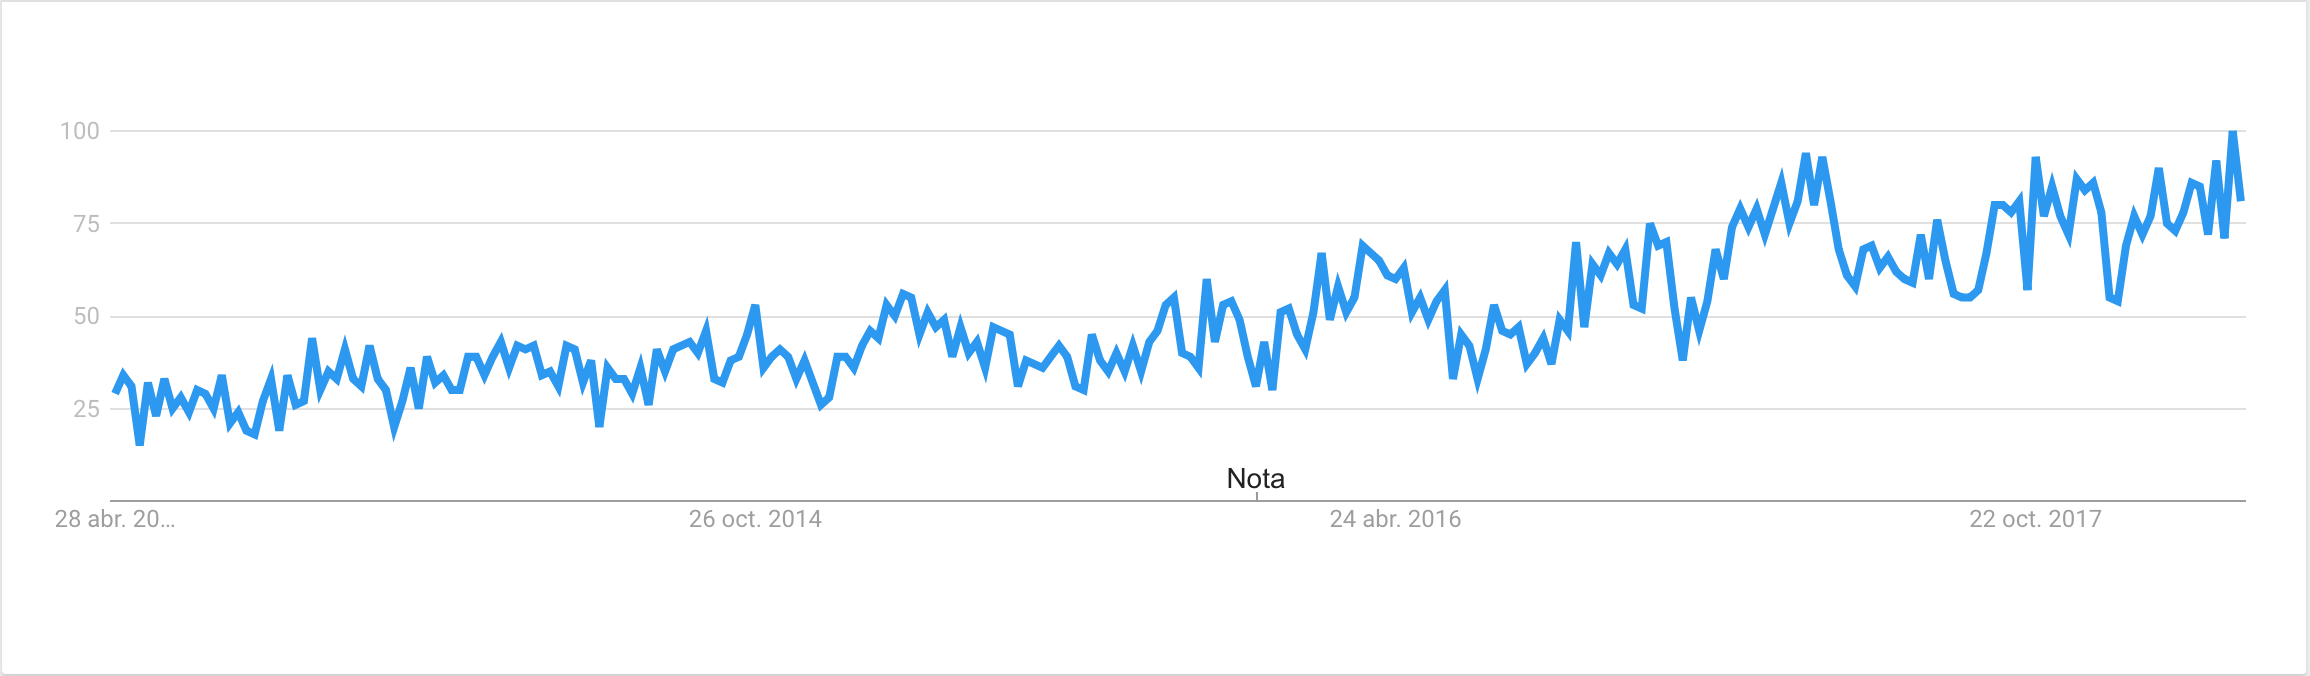
\includegraphics[width=1\linewidth]{imagenes/interes}
	 	\caption{Gráfica que representa el interés del análisis de sentimientos en todo el mundo según Google Trends.}
	 	\label{fig:interes}
	 \end{figure}
	 
	 Esto hace que se presente como una campo de estudio muy llamativo, con muchas mejoras por hacer y con un futuro muy prometedor. Cada día más gente centra su interés en esta materia (Figura \ref{fig:interes}). De ahí que a lo largo de esta memoria nos dediquemos al estudio de una parte de este amplio campo.
	 

	Como ya podemos imaginar, el término Análisis de Sentimientos abarca un gran conjunto de tareas. El trabajo se va a centrar en una de esas tareas en concreto: la extracción de características. 

	Para explicar en qué consiste y su importancia, trabajaremos sobre un ejemplo concreto. Imaginemos que queremos analizar la siguiente opinión:
	
	\begin{center}
		\begin{minipage}{0.9\linewidth}
			\vspace{5pt}%margen superior de minipage
			{\small
				[1] \textit{El ordenador tiene muy buen procesador, sin embargo la pantalla tiene poca resolución y el precio es muy elevado.}
			}
			\vspace{5pt}%margen inferior de la minipage
		\end{minipage}
	\end{center}

	Si tuviéramos que establecer una polaridad a dichar frase, sería una tarea complicada incluso para una persona. En la frase se nombran tres componentes de un mismo ordenador y se da un opinión sobre cada una de ellas. Así, \textit{buen procesador} tendría connotaciones positivas mientras que \textit{la pantalla tiene poca resolución} y \textit{el precio es muy elevado} negativas. La polaridad general del producto dependerá de la importancia que se le dé a cada una de las partes. Como no podemos saber a priori un orden de prioridad establecido, sería muy útil poder dar una polaridad a cada una de las componentes.
	
	Ahora bien, para poder realizar este proceso de forma automatizada nos encontraríamos con dos tareas: en primer lugar la identificación de la característica y, en segundo lugar, la detección de la polaridad de esta. En este trabajo nos centraremos en la primera de estas tareas. 

	\section{Objetivos} \label{objetivos}
	
	En este trabajo se pretende dar una pequeña introducción al Análisis de sentimientos, ciencia muy amplia de la que nos centraremos en resolver un tipo de problema concreto. Nuestro objetivo será resolver el problema de extracción de características.
	
	Para ponernos en contexto, realizaremos una breve introducción teórica al Análisis de sentimientos. En ella hablaremos sobre el procesamiento del Lenguaje Natural al mismo tiempo que definiremos formalmente el concepto de opinión y hablaremos de los diferentes niveles del Análisis de sentimientos donde daremos a relucir la importancia de nuestro problema concreto. 
	
	A continuación, realizaremos una introducción matemática al Deep Learning ( (?) no sé muy bien qué voy a hacer en la parte matemática) para fundamentar de forma teórica las bases de los métodos que aplicaremos en el resto del trabajo.
	
	En cuanto a la solución propuesta para resolver nuestro problema de clasificación, partiremos del modelo propuesto en el artículo de [(?) citar paper Poria]  en el que se aborda el problema con el uso de Redes Neuronales Convolutivas (CNN). Posteriormente, propondremos mejoras y/o modelos diferentes que finalmente compararemos.
	
	Así, la estructura del trabajo constaría de los siguientes tomos:
	
	 \begin{enumerate}
	 	\item Introducción teórica al Análisis de sentimientos.
	 	\item Fundamentos matemáticos del Deep Learning.
	 	\item Implementación del modelo base.
	 	\item Desarrollo de mejoras y/o nuevos modelos.
	 	\item Comparativa entre los modelos desarrollados.
	 \end{enumerate}

	 
	\section{Requerimientos}\label{requerimientos}
	
	Como ya hemos introducido en la Sección \ref{objetivos}, queremos desarrollar un software para resolver el problema de la extracción de características.
	
	Para ello, nuestro sistema aceptará un conjunto de frases con un formato determinado como entrada produciendo una secuencia de etiquetas que nos identifiquen las entidades (tanto simples como compuestas). Para ello utilizaremos el sistema de notación \textit{IOB} (IN/ OUT/ BEGING). Con este sistema, la etiqueta \textit{B} se correspondería con el inicio de una entidad. Si esta es compuesta, la siguiente palabra estaría etiquetada con la etiqueta \textit{I}. El resto de palabras que no representan una entidad serían etiquetadas con \textit{O}. 
	
	Un ejemplo de etiquetado \textit{IOB} sería el siguiente:
	
	\begin{center}
		\begin{minipage}{0.9\linewidth}
			\vspace{5pt}%margen superior de minipage
			{\small
				[1] \textit{My favourite city is New York}
				
				[2] \textit{(My, O) (favourite, O)  (city, B) (is, O) (New, B) (York, I)}
			}
			\vspace{5pt}%margen inferior de la minipage
		\end{minipage}
	\end{center}
	
	
	Para la representación de las palabras utilizaremos \textit{word embeddings} ya entrenados en diccionarios en inglés. Por lo que nuestro sistema funcionará solamente en inglés.
	

		

	



\chapter{Análisis de sentimientos}

	Para definir el concepto de Análisis de sentimientos es necesaria una breve introducción al Procesamiento del Lenguaje Natural.

\section{Procesamiento del Lenguaje Natural} \label{conceptsentiment}	
	
	 El Procesamiento del Lenguaje Natural (PLN) es un campo de la Inteligencia Artificial que se encarga de estudiar la comunicación que surge entre personas y máquinas. El objeto de estudio del PLN es, por tanto, el lenguaje. Para que las máquinas puedan conseguir capacidad de procesamiento y de generación del lenguaje, es necesario que se tenga comprensión total de la lengua. De esta misión se encarga la Lingüística, que trata de caracterizar y explicar los procedimientos del lenguaje.
	
	El procedimiento usual de un sistema PLN se divide en tres fases principales: análisis sintáctico, semántico y pragmático. En la práctica, estas fases no son suficientes. Esto se debe a que no es viable realizar el análisis sintáctico de un texto sin haber identificado las palabras y las oraciones además de la información morfológica de las palabras que componen la frase. Así, a las tres fases anteriores habría que añadir dos nuevas fases: \textit{tokenización} y análisis léxico.
	
	
	A continuación observamos el flujo de trabajo que seguiría un sistema PLN. La funcionalidad de la cada una de las fases sería:

		\begin{minipage}{.65\textwidth}
			\begin{enumerate}% never number things manually!
				\item \textit{Tokenización: }  Identificar las unidades en las que se divide el mensaje, \textit{tokens}.
				\item Análisis léxico: Obtiene información de los \textit{tokens} a partir de la función que desempeñan en la oración.
				\item Análisis sintáctico: Obtiene las relaciones y dependencias existentes entre los elementos que componen la oración.
				\item Análisis Semántico: Obtención de la intención del autor a partir de la información obtenida en la fase anterior. Busca descubrir el significado de la frase.
				\item Análisis Pragmático: Busca las conexiones entre oraciones para dar un sentido global al discurso.
			\end{enumerate}
		\end{minipage}
		\begin{minipage}{.35\textwidth}
			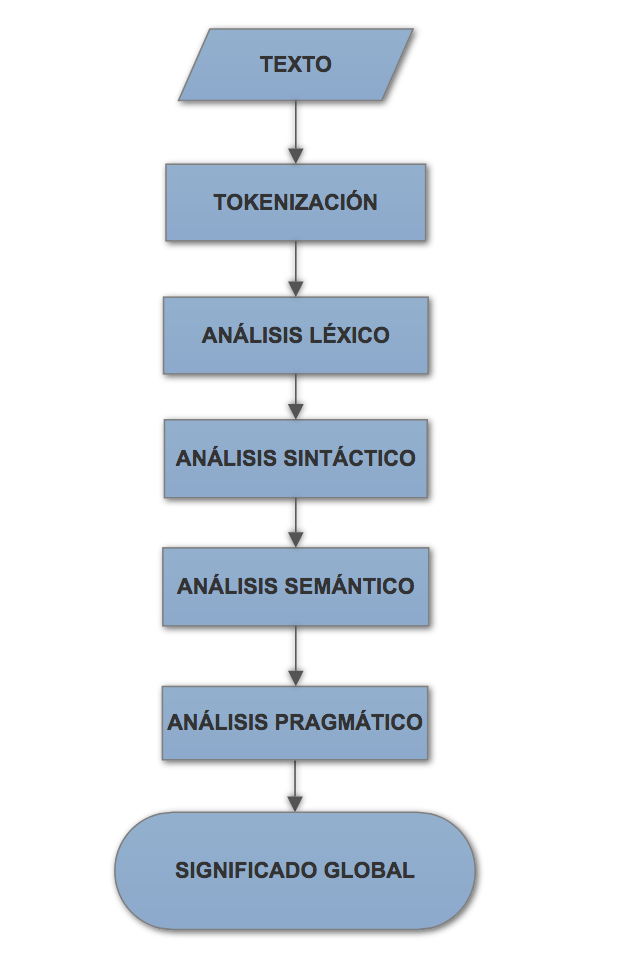
\includegraphics[width=1\linewidth]{imagenes/flujo}
		\end{minipage}
		
	La búsqueda del entendimiento del lenguaje no es la única misión del PLN. También persigue la generación automática de lenguaje, aunque no va a ser en lo que centremos esta memoria.
	
	
	
\section{Concepto de Análisis de sentimientos}\label{conceptoSA}

	El Análisis de sentimientos (AS) recibe muchos nombres dado a la evolución histórica que ha tenido: Análisis de Opiniones, Minería de Opiniones, etc. A partir de ahora y durante todo el proyecto nos referiremos a él como Análisis de sentimientos.
	
	Definimos el Análisis de sentimientos como el estudio computacional de opiniones, sentimientos y emociones expresadas en un texto. Puede ser considerado como un proceso de clasificación cuyo fin es decidir la polaridad del sentimiento expresada en el texto. La dificultad de esta ciencia recaerá en el objeto de estudio pues se trata de información desestructurada, teniendo que convertirlos en datos estructurados. 
	
	\subsection{Concepto de Opinión}\label{opinion}
	
		Como hemos comentado en la sección anterior, el objetivo del AS consite en la extracción de información a partir de textos. Fundamental para definir ese concepto será la definición de su objeto de estudio, el concepto de opinión.
		
		Una primera aproximación para la definición de opinión la encontramos en el diccionario de la RAE, una opinión es un ``juicio o valoración que se forma una persona respecto de algo o de alguien.'' De esta definición podemos destacar varias cosas. Claramente una opinión es subjetiva, juicio o valor, pero también vemos que se hace énfasis en  quién crea la opinión y sobre qué. Empezamos así a vislumbrar que la opinión estará formada por varios elementos. 
		
		Para hacer más énfasis en este concepto de opinión formada por varios elementos, veamos un ejemplo concreto:
		
			\begin{center}
			\begin{minipage}{0.9\linewidth}
				\vspace{5pt}%margen superior de minipage
				{\small
					\textit{[1] El pasado jueves fui con un grupo de amigos a cenar a un restaurante. [2] Pedí unos macarrones a la carbonara que estaban deliciosos. [3] Sin embargo, el postre no me gustó nada, pedí una tarta de queso. [4] Creo que en este sentido acertó más mi amiga María que pidió la tarta de tres chocolates, ¡le encantó! [5] En cuanto al precio, no estaba nada mal para la cantidad que servían. [6] También hay que  tener en cuenta que se encontraba a las afueras, solo se puede acceder en coche.}
				}
				\vspace{5pt}%margen inferior de la minipage
			\end{minipage}
		\end{center}
	

	Si observamos el texto anterior con la intención de extraer una opinión global sobre el restaurante, encontramos que se da información ``contradictoria'' pues hay oraciones que expresan sentimientos negativos, positivos e incluso neutros. La oración [1] expresa un hecho, sin ningún juicio de valor. Por su parte, las oraciones [2], [4] y[5] expresan sentimiento positivo mientras que las oraciones [3] y [6] expresan alguna opinión negativa. Vemos que cada una de estos juicios se realizan a ciertos elementos del restaurante, por lo que será algo a tener en cuenta dependiendo de si queremos determinar opinión de la entidad (restaurante) o de cada uno de sus componentes. Otro detalle presente en el ejemplo es que no siempre la persona que juzga algo es el autor del texto. En este caso, en la frase [4] el autor expresa que a su amiga le encantó su postre. Destacar también la importancia del tiempo a la hora de realizar un juicio de valor pues nuesta opinión puede variar a lo largo del tiempo. 
	
	En este punto, podemos considerar la opinión como una cuádrupla \textit{(o, p, h, t)} donde \textit{o} representa el objeto sobre el que recae la opinión, \textit{p} la polaridad de la misma, \textit{h} el autor y \textit{t} el tiempo en el que se produjo.
	
	Si nos fijamos en la frase [3] que expresa un sentimiento negativo, vemos que la opinión negativa no es sobre el restaurante en su conjunto si no que  es hacia un postre concreto. Según la definición de opinión como una cuádrupla \textit{(o, p, h, t)} su polaridad recaería sobre el objeto en cuestión, el restaurante. Así, surge la necesidad de considerar que el objeto pueda ser dividido en diferentes componentes. Definimos como entidad \textit{e} a un producto, servicio, tema, persona, organización o ente. Esta entidad se representa mediante \textit{(T,W)} donde \textit{T} es una jerarquía de componentes y \textit{W} el conjunto de atributos de \textit{e}. 
	
	Con esta nueva consideración llegamos a nuestra definición de opinión, introducida en \cite{liu}. Una opinión estaría formada por una quíntupla $(e_i, a_{ij}, p_{ijkl}, h_{k}, t_{l})$ donde $e_i$ representa la entidad, $a_ij$ sería el atributo de $e_i$ sobre el que recae la opinión, $p_{ijkl}$ se correspondería con la polaridad de la opinión que se hace sobre el aspecto $a_{ij}$ en el momento de tiempo $t_{l}$ por la persona $h_{k}$ y, por último, $h_{k}$ y $t_{l}$ la persona y el tiempo en que se realiza el juicio de valor respectivamente.
		 
		
	\subsection{Niveles de clasificación}\label{nivelesSA}
	
	%Aqui hacer mucho énfasis en lo importante que es hacerlo por entidades -> Dar importancia a mi trabajo
	
	Como ya hemos introducido, el objetivo final del Análisis de sentimientos es la clasificación de un texto según su polaridad. Ahora bien, a la hora de clasificar la polaridad de un texto podemos considerar tres niveles:
	
	\begin{enumerate}
		\item \textbf{Nivel de texto: } Analiza el documento completo y asigna una polaridad global al documento en su conjunto. Es el nivel más general y, por tanto, menos preciso.
		\item \textbf{Nivel de sentencias: } Detecta el sentimiento en frases. Está muy relacionado con la subjetividad ya que esta se expresa en frases y no en documentos largos. Obtendríamos uan clasificación más precisa del sentimiento.
		\item \textbf{Nivel de aspectos o entidades: } Detecta el sentimiento u opinión y la entidad a la que se refiere. Es el nivel más preciso de análisis, pues no produce generalizaciones si no que se identifica una polaridad con un aspecto concreto.
	\end{enumerate}
	
	 Como ya hemos comentado, nuestro proyecto se centrará en el último de estos niveles de clasificación. La importancia de esta especificación queda reflejada en el ejemplo que pusimos en la sección \ref{opinion}. Además, una vez tengamos clasificada la polaridad de los diferentes aspectos o entidades, es fácilmente extrapolable al resto de niveles de clasificación. Podemos obtener la clasificación a nivel de sentencias simplemente con la combinación de la polaridad de cada uno de los aspectos que aparecen en la sentencia y análogamente con la clasificación a nivel de texto.
\chapter{Fundamentos matemáticos}

\textcolor{red}{Concepto de derivada y definiciones alternativas.}

\textcolor{red}{Uso de la derivada en minimización de funciones.}

\textcolor{red}{Gradiente para una función en Rn}

\textcolor{red}{Composición de funciones.}

\textcolor{red}{Grafos dirigidos.}

\textcolor{red}{ÁLGEBRA TENSORIAL -- Optimización de algoritmos deeplearning (tensorflow)}

\textcolor{red}{PROBABILIDAD y TEORIA DE LA INFORMACION}
		
		- entropia cruzada -- log-verosimilitud negativa

\section{Probabilidad} \label{prob}

 - dist probabilidad
 
 - estadistico -- inferencia
 
\chapter{Aprendizaje Automático}

	En este capítulo desarrollaremos los principios básicos de aprendizaje automático para introducir el \textit{Deep Learning} en capítulos posteriores. Motivaremos su uso con algunos ejemplos y nos adentraremos en el problema de clasificación pues es el que desarrollaremos durante el resto de la memoria. 
erosi	
	Finalmente hablaremos del gradiente descendente, algoritmo de optimización en el cual se inspirará el Deep Learning.
	
	
\section{Concepto de Aprendizaje Automático}\label{introap}

	Un algoritmo de \textbf{Aprendizaje Automático} es un algoritmo que es capaz de aprender información a partir de ciertos datos.  Pero, ¿qué entendemos por aprender? Según \cite{mitchell}, ``Un programa de ordenador se dice que aprende de una experiencia \textit{E} con respecto a un conjunto de tareas \textit{T} y medida de rendimiento \textit{P}, si su rendimiento como tarea en \textit{T}, medido con \textit{P}, mejora tras conocer la experiencia \textit{E}''. Como podemos imaginar, estas tareas y experiencias son muy diversas, de donde surgen gran variedad de técnicas de aprendizaje con estas características.
	
	Desde  el punto de vista de las tareas \textit{T}, el aprendizaje automático es interesante pues nos permite tratar con tareas que son muy difíciles de resolver con programas escritos y diseñados por humanos, ya sea por la complejidad de la solución o por el tamaño de la tarea.
	
	Han sido muchas las aplicaciones de esta clase de algoritmos. En la literatura podemos encontrar varios ejemplos:
	
	\begin{itemize}
		\item Clasificación
		\item Clasificación con valores perdidos
		\item Regresión
		\item Transcripción
		\item Detección de anomalías
		\item Predicción de valores pedidos
		\item Estimación de densidad
	\end{itemize}
	
	Con respecto a la medida de rendimiento, \textit{P}, debemos diseñar una medida cuantitativa. La medida por excelencia para casos de clasificación y transcripción es la exactitud o \textit{accuracy} de la solución, definida como la proporción de muestras para las que el modelo ha producido una salida correcta. También puede ser útil en algunos casos la tasa de error o \textit{error rate}, que mide la proporción de muestras para las que el modelo ha producido uan salida incorrecta. 
	
	Para aquellas tareas como la estimación de densidad, en las que la salida es continua no tiene sentido utilizar las medidas anteriormente comentadas. En estos casos se utilizarán medidas que proporcionen resultados continuos.
	
	\subsection{Tipos de aprendizaje automático.}
	
	En función de la experiencia \textit{E}, podemos clasificar los algoritmos de aprendizaje automático en dos grandes grupos: algoritmos supervisados y no supervisados.
	
	
	\begin{itemize}
		\item \textbf{Aprendizaje Automático no supervisado}: hablamos de este tipo de aprendizaje cuando los datos con los que trabajamos se conforman de un conjunto de datos que representan diferentes características de cada una de las muestras. De este modo, el objetivo suele ser encontrar propiedades importantes para la estructura del conjunto de datos. Un ejemplo clásico de problema de este tipo es el \textit{clustering}, que consiste en la agrupación de los datos en diferentes subconjutnos que contengan características similares.
		
		\item \textbf{Aprendizaje Automático supervisado}: se obtiene información de un conjunto con características pero donde cada muestra tiene asociada una etiqueta. Así, el objetivo de este tipo de problemas es encontrar una relación entre la etiqueta y las características, pudiendo etiquetar muestras futuras. Un ejemplo de este tipo de problema es la clasificación, en el que entraremos en más detalle a continuación.
	\end{itemize}

	Prácticamente todo el Deep Learning está motivado por el \textbf{Gradiente Descendente Estocástico}. Este algoritmo es una extensión del Gradiente Descendente. Por tanto, a continuación haremos una breve introducción a estos dos conceptos.
	
	
	\section{Problema de clasificación}
	
	\textcolor{red}{Encontrar referencia formal donde pueda yo explicar esto}
	
	\section{Optimización basada en Gradiente Descendente}
	
	La mayoría de los algoritmos de Deep Learning involucran algún tipo de optimización. La función que queremos optimizar $f(x)$ se denomina \textbf{función objetivo}. 
	
	Suponemos que tenemos una función $y = f(x)$ con $x,y \in \mathbb{R}$. La derivada de esta función, $f'(x)$ nos el crecimiento/decrecimiento de la misma. Es decir, nos indica cómo escalar un pequeño cambio en la entrada, para obtener el correspondiente cambio en la salida. Esto es, usando la definición clásica de derivada con valores muy pequeños de $\epsilon$:
	
	$$
		f'(x) = \lim_{\epsilon \rightarrow 0} \frac{f(x+ \epsilon) - f(x)}{\epsilon} \Rightarrow f(x+ \epsilon) \approx f(x) + \epsilon f'(x)
	$$
	
	De este modo podríamos minimizar la funciñon $f$ pues sabríamos cómo variar $x$ para realizar una mejora en $y$. Por ejemplo, si $f(x - \epsilon$sign$(f'(x))) < f(x)$ para $\epsilon > 0$ arbitrario, entonces podemos reducir $f(x)$ sin más que mover $x$  en el sentido contrario al signo de la derivada. Esta técnica es lo que se conoce como gradiente descendente para una variable. 
	
	En el caso de varias variables, el procedimiento es muy similar. Consideraremos el gradiente de la función $f: \mathbb{R^n} \rightarrow \mathbb{R}$ en $x$, $\nabla_x f(x)$ y nos movemos una cantidad $\epsilon > 0$ en misma dirección y sentido contrario de la forma:
	
	$$
		x' = x - \epsilon \nabla_x f(x)	
	$$ 

	El algoritmo multivariante termina cuando $\nabla_x f(x)$ es 0 o muy cercano según una tolerancia prefijada.
	
	Destacar que la velocidad con la que avance el método variará en función del valor tomado para $\epsilon$ en ambos casos. Así, si elegimos un valor de $\epsilon$ muy pequeño, el método puede avanzar de forma demasiado lenta mientras que si elegimos un valor muy alto puede producirse un efecto \textit{zigzag} alrededor de un óptimo local
	
	\textcolor{red}{Ejemplos?}

	\subsection{Gradiente Descendente Estocástico}
	
	Un problema del Aprendizaje Automático radica en que para obtener suficiente generalización, el conjunto de datos sobre el que entrenamos los datos debe ser lo suficientemente grande. Esto conlleva una carga muy elevada de cómputo, pues normalmente la función de coste se calcula como la suma del valor en cada uno de los valores de la muestra.
	
	El Gradiente Descendente Estocástico (GDS) se basa en la idea de subsanar este problema utilizando solo un conjunto pequeño de muestras, llamado \textbf{minibatch} $\mathbb{B} = \{x^{(1)}, ..., x^{(m)}\}$, donde $m$ representa una pequeña muestra en función con el total del conjunto de datos.
	
	De esta forma, la estimación del gradiente sería
	
	$$ 
		g = \frac{1}{m} \nabla_{\theta} \sum_{i = 1}^{m} L(x^{(i)}, y^{(i)}, \theta)
	$$
	
	donde $x \in \mathbb{B}$. A continuación, mediante el algoritmo del Gradiente Estocástico descendente se estimaría el gradiente de la siguiente forma
	
	$$ 
		\theta \leftarrow \theta - \epsilon g
	$$
	
	donde $\epsilon$ es la tasa de aprendizaje.
	
	
	El Deep Learning se ve motivado porque el Aprendizaje Automático no había conseguido resolver los problemas centrales de la Inteligencia Artificial, como por ejemplo el reconocimiento de imágenes o procesamiento natural del lenguaje.
	



\chapter{Deep Learning}

	En este capítulo nos centramos en las técnicas implementadas a lo largo de la memoria, técnicas de \textit{Deep Learning}. Los diferentes modelos que implementaremos se basan en redes neuronales, por lo que dedicaremos la primera sección de este capítulo a hablar sobre redes neuronales prealimentadas. También se tratarán las características generales de las redes neuronales que nos servirán como base introductoria de los modelos desarrollados.
	
	A continuación, desarrollaremos en profundidad los modelos implementados: redes neuronales convolucionales y redes neuronales recursivas (LSTM). 
	
	%Por último, daremos una justificación teórica del comportamiento de estos modelos en el problema concreto que estamos tratando.

\section{Redes Neuronales Prealimentadas}

Las \textbf{redes neuronales} son el ejemplo más típico de modelos de \textit{Deep Learning}. El objetivo de esta clase de algoritmos es aproximar una función $f^*$. Por ejemplo, para un clasificador $y = f^*(x)$ que asocia a cada entrada $x$ una categoría $y$. Así, una red neuronal prealimentada define una asociación $y = f(x; \theta)$ y aprende los valores de los parámetros $\theta$ que ofrecen la mejor aproximación de la función.

Esta clase de modelos se llaman \textbf{prealimentados} porque la información fluye a través de la función siendo evaluados desde $x$, mediante los cálculos intermedios usados para definir $f$ y finalmente hasta la salida $y$. Por tanto, nunca se forman ciclos entre las conexiones de las unidades, la información se evalúa siempre hacia delante a través de las diferentes capas intermedias. No existe ningún tipo de retroalimentación en las que la salida de alguna capa de la red vuelva a ser entrada del modelo. 

Las redes neuronales son llamadas \textbf{redes} pues se definen mediante la composición de diferentes funciones. Este modelo de sucesivas composiciones se puede ver como un grafo dirigido acícilo.  

El número de capas que tenga la red definen la \textbf{profundidad} del modelo. Las capas se van nombrando de forma sucesiva siendo la primera la primera capa o \textit{capa de entrada}, \textit{segunda capa}, y así sucesivamente hasta la capa final denominada \textit{capa de salida}. El objetivo del modelo es conducir la función de entrada $f(x)$ para que se ajuste a $f^*(x)$. 

Este tipo de algoritmos están inspirados en la neurociencia, en concreto en las neuronas de los seres vivos. Cada capa del modelo está formado por un número de unidades. El número de unidades en cada capa define la \textbf{anchura} del modelo. Cada una de estas unidades que actúa de forma paralela, representa una neurona que recibe información de otras unidades (neuronas) y calcula su propio valor de activación. 

\begin{figure}[h!]
	\centering
	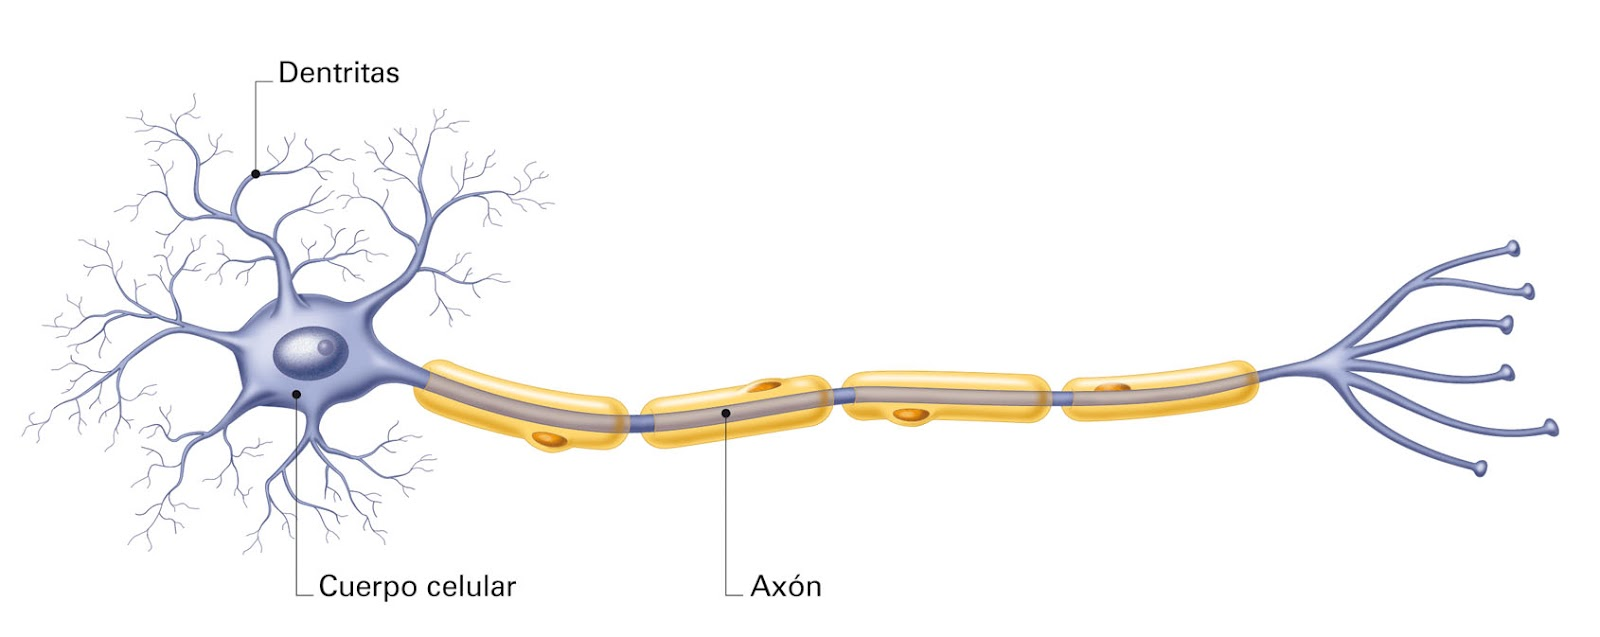
\includegraphics[width=0.7\linewidth]{imagenes/Neurona}
	\caption{Representación de una neurona biológica.}
	\label{fig:neurona}
\end{figure}


El símil con las neuronas de los seres vivos es que estas se componen de dentritas que se encargan de recoger los estímulos de otras neuronas (entradas), un núcleo para su almacenamiento (activación) y un axón con terminales que le permiten transmitir los impulsos a otras neuronas (salidas).

\begin{figure}[h!]
\centering
\begin{tikzpicture}[
init/.style={
	draw,
	circle,
	inner sep=2pt,
	join = by -latex
},
squa/.style={
	draw,
	inner sep=2pt,
	join = by -latex
},
start chain=2,node distance=13mm
]
\node[on chain=2, init] 
(x2) {$x_2$};
\node[on chain=2,join=by o-latex] 
{$w_2$};
\node[on chain=2,init ,label={[label distance=0.75cm]below:Activación}] (sigma)
{$ g(w^tx + b)$};
\node[on chain=2, init ,label={[label distance=1.5cm]below:Salida}](y)
{$y$};
\begin{scope}[start chain=1]
\node[on chain=1, init] at (0,1.5cm) 
(x1) {$x_1$};
\node[on chain=1,join=by o-latex] 
(w1) {$w_1$};
\end{scope}
\begin{scope}[start chain=3]
\node[on chain=3, init ,label=below:Entradas] at (0,-1.5cm) 
(x3) {$x_3$};
\node[on chain=3,join=by o-latex,label=below:Pesos] 
(w3) {$w_3$};
\end{scope}

\draw[-latex] (w1) -- (sigma);
\draw[-latex] (w3) -- (sigma);
\draw[-latex](sigma) -- (y);

\end{tikzpicture}
\caption{Representación de una neurona artificial de 3 entradas con función de activación g.}
\label{fig:neuron_articial}
\end{figure}

La neurona artificial se define como en la Figura \ref{fig:neuron_articial}, donde identificamos una neurona biológica con una función $f: \mathbb{R}^n \rightarrow \mathbb{R}$ donde $n$ es el número de unidades en la capa anterior (entradas).

En conclusión, una red neuronal artifical estaría formada por un número arbitrario de capas y un número arbitrario de unidades (neuronas artificiales) en cada capa. 

\begin{figure}[h!]
	\centering
	\begin{tikzpicture}[
	init/.style={
		draw,
		circle,
		font = \Large,
		inner sep=2pt,
		join = by -latex
	},
	squa/.style={
		draw,
		inner sep=2pt,
		join = by -latex
	},
	start chain=2,node distance=13mm
	]
	\node[on chain=2, init] 
	(x2) {$x_2$};
	

	\begin{scope}[start chain=1]
		\node[on chain=1, init] at (0,1.5cm) 
		(x1) {$x_1$};
	\end{scope}
	
	\begin{scope}[start chain=3]
		\node[on chain=3, init ,label={[label distance=2cm]below:Entradas}] at (0,-1.5cm) 
		(x3) {$x_3$};
	\end{scope}
	
	\begin{scope}[start chain=4]
	\node[on chain=3, init] at (1.5,3cm) 
	(h1) {$h_1$};
	\end{scope}
	
	\begin{scope}[start chain=5]
	\node[on chain=3, init] at (1.5, 1cm) 
	(h2) {$h_2$};
	\end{scope}
	
	\begin{scope}[start chain=6]
	\node[on chain=3, init] at (1.5,-1cm) 
	(h3) {$h_3$};
	\end{scope}
	
	\begin{scope}[start chain=7]
	\node[on chain=3, init,label={[label distance=0.5cm]below:Capa oculta}] at (1.5,-3cm) 
	(h4) {$h_4$};
	\end{scope}
	
	\begin{scope}[start chain=8]
		\node[on chain=8,init, label= {[label distance=3.6cm]below:Salida}] at (7,0 cm) (sigma)
	{y};
	\end{scope}
	
	
	
	\draw[-latex] (x1) -- (h1);
	\draw[-latex] (x1) -- (h2);
	\draw[-latex] (x1) -- (h3);
	\draw[-latex] (x1) -- (h4);
	\draw[-latex] (x2) -- (h1);
	\draw[-latex] (x2) -- (h2);
	\draw[-latex] (x2) -- (h3);
	\draw[-latex] (x2) -- (h4);
	\draw[-latex] (x3) -- (h1);
	\draw[-latex] (x3) -- (h2);
	\draw[-latex] (x3) -- (h3);
	\draw[-latex] (x3) -- (h4);

	\draw[-latex](h1) -- (sigma);
	\draw[-latex](h2) -- (sigma);
	\draw[-latex](h3) -- (sigma);
	\draw[-latex](h4) -- (sigma);
	
	\end{tikzpicture}
	\caption{Representación de una neurona artificial de 3 entradas con función de activación g.}
	\label{fig:rrnn_artifical}
\end{figure}

  
Observamos en la Figura \ref{fig:rrnn_artifical} un ejemplo simplificado de una red neuronal con tres capas: capa de entrada, una capa oculta y capa de salida. La capa de entrada tiene tres unidades, la oculta cuatro y la de salida una.

Una forma de entender las redes neuronales prealimentadas es conocer las limitaciones de los modelos lineales y considerar cómo superarlas. El éxito de los modelos lineales como la regresión logística o lineal radica en su eficiencia y fiabilidad. Sin embargo, no se puede  ignorar el  inconveniente de que están limitados a funciones lineales, por tanto no contemplan las posibles relaciones entre dos variables de entrada.

Para extender estos modelos de forma que representen funciones no lineales de $x$, podemos considerar un modelo lineal sobre una transformación de la entrada $\phi(x)$ donde $\phi$ es una transformación no lineal. El problema se traduce, entonces, en encontrar qué transformación no lineal $\phi$ aplicar a la entrada $x$:

\begin{itemize}
	\item La primera opción sería estudiar manualmente qué función se ajusta más al problema concreto, lo que conllevaría un alto conocimiento del problema.
	\item Otra opción sería utilizar una función genérica $\phi$ de alta dimensionalidad para que siempre tenga la suficiente capacidad de adaptarse al conjunto de entrenamiento, lo cual no proporciona una buena generalización en el conjunto de test.
	\item El enfoque que aporta el \textit{deep learning} es aprender $\phi$ en un conjunto de funciones parametrizadas. Así, tenemos el modelo 
	$$y = f(x; \theta, w) = \phi(x; \theta)^T w$$ 
	
	donde $\theta$ es un conjunto de parámetros utilizado para aprender $\phi$ de entre la clase de funciones consideradas. 
\end{itemize}

	Este modelo nos aporta una gran flexibilidad pues la elección de la función de transformación depende del conjunto de funciones que estemos considerando. Además, al igual que en los modelos lineales deberemos predefinir ciertos aspectos de diseño: optimizador, función de coste y forma de las unidades de salida. Las redes neuronales prealimentadas introducen el concepto de capa oculta, por lo que tendremos que elegir también las funciones de activación que se utilizarán para calcular la salida de cada una de estas capas. También será necesario definir la arquitectura de la red, definiendo cuántas capas añadir y cuántas unidades tendrá cada una.  
	
	A continuación estudiaremos algunas de las funciones comentadas.
	
	\subsection{Función de coste}
	
	La principal diferencia entre los algoritmos lineales y las redes neuronales es la ya comentada no linealidad. Esta característica hace especialmente interesante considerar funciones de coste no convexas en este tipo de modelos. 
	
	Aunque en algunos casos podemos definir la función de coste como un estadístico de $y$ condicionado a $x$. En la mayoría de los diseños, el modelo paramétrico definido define una distribución de probabilidad $ p(y | x ; \theta)$ y podemos aplicar el principio de máxima verosimilitud comentado en la Sección \ref{prob}. Esto significa que usamos la entropía cruzada entre los datos de entrenamiento y las predicciones del modelo como función de coste:
	
	$$
		J(\theta) = - \mathbb{E}_{x,y \sim \hat{p}_{data}} \log p_{model}(y | x)
	$$
	
	La ventaja de esta función de coste es que queda determinada en función de $p_{model}(y|x)$ ahorrándonos el trabajo de definir una función de coste propia para cada problema. Además, un tema recurrente en el diseño de redes neuronales es que el gradiente de la función de coste debe ser grande para evitar que el valor del gradiente vaya rápidamente a cero y nuestra función de coste cumple este requisito.
	
	
	\subsection{Unidades de salida}
	
	La elección de la función de coste está estrechamente relacinada con la elección de la unidad de salida. La mayoría de las veces simlpemente utilizamos la entropía cruzada de la distribución de los datos y de la distribución del modelo.
	
	Aunque en esta sección nos centremos en unidades de salida, estas funciones pueden ser	utilizadas en las capas ocultas también. Para unificar la  notación supondremos que la red neuronal produce una salida de las capas ocultas definida por el vector de características $h = f(x; \theta)$. 
	
	Aunque existen muchas posibiildades, las principales unidades de salida son de los siguientes tipos:
	
	\subsubsection{Unidades lineales}
		
		Un tipo de unidad de salida está basada en una transformación lineal. Esto es, dado el vector de características $h$, la capa produce como salida el vector 
		
		$$
			\hat{y} = W^Th + b
		$$ 
		
		El uso principal de este tipo de unidades de salida es producir la media de una distribución condicional normal:
		
		$$
			p(y | x) = \mathcal{N}(y; \hat{y}, I)
		$$ 
		
		Para esta probabilidad condicionada concreta, calcular la entropía cruzada (log-verosimilitud negativa) es equivalente a minimizar usando el error cuadrático medio.
		
	\subsubsection{Unidades sigmoidales}
	
		Este tipo de unidades se utilizan para tareas que requieren la predicción de una variable binaria $y$. La probabilidad condicionada aplicada en la técnica de máxima verosimilitud en este caso se correspondería con la definición de una distribución de Bernouilli sobre $y$ condicionada a $x$. Esta distribución se define con un número en el intervalo [0,1] determinado por la probabilidad  $P(y = 1 | x)$.
		
	\subsubsection{Unidades con activación softmax}
		
		

	
\section{Redes Neuronales Convolucionales}



\section{Redes Neuronales Recurrentes}

\subsection{Long-Short Term Memory}
\chapter{Redes Neuronales Convolucionales}\label{cnn}

	Las Redes Neuronales Convolucionales o \textit{CNN} son un tipo especializado de red neuronal para el procesamiento de datos con estructura de cuadrícula específica. 
	
	Durante el capítulo describiremos la operación matemática en la que se basan este tipo de redes, conocida como convolución. Posteriormente describiremos otra operación que suelen implementar este tipo de redes, el \textit{pooling}. 
	
	
	\section{La operación de Convolución}
	
	Una convolución es una operacion en dos funciones de argumentos en $\mathbb{R}$ generando una tercera función combinando las dos anteriores. 
	
	Dadas dos funciones que toman valores reales $f, g: \mathbb{R} \rightarrow \mathbb{R}$ con la regularidad necesaria, se denota como $(f \ast g)$ y se define como el producto de ambas funciones habiendo previamente invertido y desplazado una de ellas. Esto es:
	
	$$
		s(t) =	(f \ast g)(t) = \int_{- \infty}^{\infty} f(s) g(t-s) ds
	$$	
	
	En la terminología de las redes neuronales convolucionales, el primer argumento ($f$) es conocido como \textbf{entrada}  y el segundo ($g$) como \textbf{núcleo}. La salida se denomina \textbf{mapa de características}. 
	
	 Para la definición de convolución hemos supuesto $f$ y $g$ funciones continuas definidas en $\mathbb{R}$. Sin embargo, esta condición de proporcionar valores en cada instante de tiempo (de forma continua) no es realista. Cuando trabajamos con datos en un ordenador, el tiempo se discretiza y nuestras funciones pasarían a tomar valores de forma discreta. Para ello, definimos la \textbf{función de convolución discreta,} que será la utilizada por las redes neuronales convolucionales de la siguiente manera:
	 
	 $$
		 s(t) =	(f \ast g)(t) = \sum_{s = - \infty}^{\infty} f(s) g(t-s) 
	 $$
	 
	En los modelos de aprendizaje, la entrada suele ser un vector multidimensional de datos y el núcleo un vector multidimensional de parámetros que se adaptan mediante el algoritmo de aprendizaje. Supondremos que las funciones toman valor 0 en todo su dominio menos en el conjunto finito de puntos que se almacenan como valores. Esto significa que, en la práctica, podemos implementar la suma infinita de la definición como una suma finita de elementos ignorando aquellos elementos que sumen una cantidad nula.
	
	Normalmente se utilizan más de una convolución al mismo tiempo en diferentes ejes. 
	
	Por ejemplo, si consideramos una imagen bidimensional $I$ como entrada, podríamos aplicar un núcleo bidimensional $K$ de la siguiente manera:
	
	
	$$
		S(i,j) = (I \ast K)(i,j) = \sum_{m} \sum_{n} I(m,n)K(i-m, j-n) =  \sum_{m} \sum_{n} K(m,n) I(i-m, j-n)
	$$
	
	\subsection{Ejemplo de convolución}
	
	En esta subsección veremos un ejemplo de convolución sencilla para entender mejor su funcionamiento. 
	
	Por ejemplo, consideremos el último caso estudiado en la sección anterior. Tenemos una imagen bidimensional $I \in \mathcal{M}_{nxm}(\mathbb{R}) = \mathcal{M}_{5x5}(\mathbb{R})$ y aplicamos un filtro $K$ de dimensiones $(i, j) = (2,3)$ en los respectivos ejes. El resultado sería entonces un mapa de características de dimensiones $(n-i+1, m-j+1) = (4, 3)$.
	
	Veamos el funcionamiento de la convolución gráficamente. Tenemos la siguiente entrada:
	
	\begin{center}
		\begin{TAB}(e,1.5cm,1.5cm){|c:c:c:c:c|}{|c:c:c:c:c|}
		
			\textcolor{red}{$I_{(1,1)}$} & \textcolor{red}{$I_{(1,2)}$} & $I_{(1,3)}$& $I_{(1,4)}$&$I_{(1,5)}$\\ 
			\textcolor{red}{$I_{(2,1)}$}& \textcolor{red}{$I_{(2,2)}$}&  $I_{(2,3)}$& $I_{(2,4)}$ &$I_{(2,5)}$\\ 
			\textcolor{red}{$I_{(3,1)}$}&  \textcolor{red}{$I_{(3,2)}$}&  $I_{(3,3)}$&    $I_{(3,4)}$ &    $I_{(3,5)}$ \\ 
			$I_{(4,1)}$&  $I_{(4,2)}$ &  $I_{(4,3)}$&    $I_{(4,4)}$ &    $I_{(4,5)}$ \\
			$I_{(5,1)}$&  $I_{(5,2)}$ &  $I_{(5,3)}$&    $I_{(5,4)}$ &    $I_{(5,5)}$  
		\end{TAB}
	\end{center}

	Tras aplicar la convolución con las dimensiones del núcleo indicadas, denotando a $S$ como la función convolución tenemos:

	\begin{center}
		\begin{TAB}(e,1.5cm,1.5cm){|c:c:c:c|}{|c:c:c|}
		 \textcolor{red}{S(1,1)} & S(1,2) & S(1,3)& S(1,4)\\
		 S(2,1)& S(2,2) & S(2,3)& S(2,4)\\
		 S(3,1)& S(3,2) & S(3,3)& S(3,4)
		\end{TAB}
	\end{center}

	donde $S(1,1) = f(I_{(1,1)}, I_{(1,2)}, I_{(2,1)}, I_{(2,2)}, I_{(3,1)}, I_{(3,2)})$ y así sucesivamente.
	
	\section{\textit{Pooling}}
	
	Una típica capa de una red neuronal consiste en tres pasos:
	
	\begin{enumerate}
		\item La capa realiza varias convoluciones en paralelo para producir un conjunto de activaciones lineales.
		\item Al resultado de cada activación lineal se le aplica una función de activación no lineal. 
		\item Se usa una función de \textit{pooling} para modificar aúm más la salida de la capa.
	\end{enumerate}

	Una función de \textit{pooling} reemplaza la salida de la red en una determinada localización con valores estadísticos de las salidas cercanas. Como ejemplos de funciones de \textit{pooling} podemos destacar el \textbf{\textit{max pooling}} que devuelve el máximo de un vecindario rectangular, o aquella que devuelve la media o la norma $\mathcal{L}^2$ de vecindarios rectangulares.
	
	En todos los casos, el aplicar \textit{pooling} hace la representación prácticamente invariante frente a pequeñas variaciones en la entrada, consiguiendo más capacidad de generalización. 
	
	\section{Adaptación a procesamiento de datos secuencial}	
	

\chapter{Modelado de secuencias: Redes Neuronales Recurrentes}
Al igual que en el capítulo anterior, en este vamos a desarrollar una clase concreta de redes neuronales, las redes neuronales recursivas y recurrentes. Esta familia de redes neuronales se utilizan para el procesamiento de datos secuencial, por lo que será natural su uso en el problema que se trata en este proyecto. 

\section{Motivación}

La innovación con respecto a las redes neuronales convencionales será el aplicar a estas nuevas técnicas de \textit{deep learning} una de las primeras ideas que surgieron en el aprendizaje automático y los modelos estadísticos: compartir los parámetros a lo largo de todo el aprendizaje. El hecho de compartir parámetros durante el aprendizaje del modelo hará posible la extensión y aplicación del modelo a ejemplos de diferentes longitudes y generalizar a través de ellos. 

Podemos entender la importancia del hecho de compartir parámetros durante el modelo en un ejemplo sencillo de procesamiento del lenguaje natural. Supongamos las frases [1] y [2]:

	\begin{center}
	\begin{minipage}{0.4\linewidth}
		\vspace{5pt}%margen superior de minipage
		{\small
			\textit{[1] Estuve en  Nepal en 2017.}
			\\\textit{[2] En 2017 estuve en Nepal.}
		}
		\vspace{5pt}%margen inferior de la minipage
	\end{minipage}
\end{center}

Si quisiéramos diseñar un algoritmo de aprendizaje automático que reconociera en qué año estuvo el narrador en Nepal, debería de reconocerse el año 2017 como la parte importante de información, independientemente de que aparezca en la quinta o en la segunda palabra de la oración. Una red neuronal tradicional usaría parámetros independientes para cada entrada, por lo que necesitaría aprender todas las reglas del lenguaje de forma independiente para cada posición en la frase. Este problema se solventaría considerando una red neuronal recurrente que comparta los mismos pesos a lo largo de todos los pasos necesarios durante el aprendizaje.

Para simplificar la notación durante el capítulo consideraremos que la red actúa sobre una secuencia que contiene vectores $x^{(t)}$ aunque en la práctica las redes suelen operar sobre conjuntos de ellas (\textit{minibatches}).

Al igual que en capítulo \ref{cnn} se definía la estructura del modelo de las redes neuronales convolucionales como un grafo acíclico, la recurrencia de este tipo de redes ampliará el concepto a grafos cíclicos. Estos ciclos representarán la influencia del valor actual de la variable en su propio valor en el siguiente paso del aprendizaje. 

\section{Despliegue de Grafos Computacionales}

	Un \textbf{grafo computacional } es una forma de formalizar la estructura de un conjunto de cálculos, como aquellos que involucran un conjunto de entradas y parámetros para producir una salida y pérdida.
	
	En esta sección desarrollaremos la idea de \textbf{desplegar} un cálculo recurrente en un grafo computacional con su correspondiente estructura de cadena de eventos. 
	
	Por ejemplo, consideramos la fórmula clásica de un sistema dinámico:
	
	\begin{equation}\label{recursive}
		s^{(t)} = f(s^{(t-1)}; \theta)
	\end{equation}
		
	
	donde $s^{(t)}$ es el estado del sistema.
	
	Es claro que esta fórmula es recurrente porque en la definición de un estado concreto de $s$ en el tiempo $t$ se utiliza el valor del mismo estado en el momento de tiempo $t-1$.
	
	Si consideramos un número de pasos finito $\tau$, el grafo puede ser desplegado aplicando la definición $\tau -1 $ veces.  Por ejemplo, para $\tau = 3$ tenemos:
	
	\begin{equation}\label{recursive2}
		s^{(3)} = f(s^{(2)}; \theta) = f(f(s^{(1)}; \theta); \theta)
	\end{equation}
		
	
	Desplegando sucesivamente la fórmula con la definición de $s$ hemos obtenido una expresión que no involucra recurrencia y que puede ser expresada con un gráfico acíclico. De esta forma el grafo para la fórmula \ref{recursive2} sería:
	
\begin{figure}[h!]
	\centering
	\begin{tikzpicture}[
	init/.style={
		draw,
		circle,
		font = \Large,
		inner sep=2pt,
		join = by -latex
	},
	squa/.style={
		draw,
		inner sep=2pt,
		join = by -latex
	},
	start chain=2,node distance=13mm
	]
	
	\node[on chain=2, init] 
	(s1) {$s^{(1)}$};
	
	\begin{scope}[start chain=3]
		\node[init] at (3, 0cm)  
		(s2) {$s^{(2)}$};
	\end{scope}
	
	\begin{scope}[start chain=4]
	\node[init] at (6, 0cm)  
		(s3) {$s^{(3)}$};
	\end{scope}
	
	\draw[-latex] (s1) -- (s2);
	\draw[-latex] (s2) -- (s3);
	
	\end{tikzpicture}
	\label{fig:recursive2}
\end{figure}

\vspace{0.5cm}

	Y de forma genérica, para la fórmula \ref{recursive} tendríamos el siguiente grafo
	
\vspace{0.5cm}

\begin{figure}[h!]

	\centering
\begin{tikzpicture}[
init/.style={
	draw,
	circle,
	minimum size=1.3cm,
	inner sep=2pt,
	join = by -latex
},
squa/.style={
	draw,
	inner sep=2pt,
	join = by -latex
},
start chain=2,node distance=13mm
]

\node[on chain=2, init] 
(s1) {$s^{(...)}$};

\begin{scope}[start chain=3]
\node[init] at (3, 0cm)  
(s2) {$s^{(t-1)}$	};
\end{scope}

\begin{scope}[start chain=4]
\node[init] at (6, 0cm)  
(s3) {$s^{(t)}$};
\end{scope}

\begin{scope}[start chain=5]
\node[init] at (9, 0cm)  
(s4) {$s^{(t+1)}$};
\end{scope}

\begin{scope}[start chain=6]
\node[init] at (12, 0cm)  
(s5) {$s^{(...)}$};
\end{scope}

\draw[-latex, dashed] (s1) -- (s2);
\draw[-latex] (s2) -- (s3);
\draw[-latex] (s3) -- (s4);
\draw[-latex, dashed] (s4) -- (s5);

\end{tikzpicture}
\label{fig:recursive}
\end{figure}

\vspace{0.5cm}

La mayoría de las redes neuronales recurrentes utilizan la fórmula \ref{hidden} para definir el valor de salida de las capas ocultas. 

\begin{equation}\label{hidden}
	h^{(t)} = f(h^{(t-1)}, x^{(t)}; \theta)
\end{equation} 
	
Cuando una red neuronal recurrente se entrena para una tarea que requiere predecir un resultado a partir de unos datos, aprende usando $h^{(t)}$ como un tipo de resumen de pérdida de los aspectos relevantes para la tarea de la secuencia de entradas hasta el momento $t$. 

\vspace{0.5cm}

La ecuación \ref{hidden} se puede representar de dos formas diferentes:
\begin{enumerate}
	\item Considerando un nodo por cada uno de los estados por los que pasa cada una de las variables del modelo como en la Figura \ref{fig:forma1}.
	
	\begin{figure}[h!]
		\centering
		\begin{tikzpicture}[
		init/.style={
			draw,
			circle,
			minimum size=1.3cm,
			inner sep=2pt,
			join = by -latex
		},
		squa/.style={
			draw,
			inner sep=2pt,
			join = by -latex
		},
		start chain=2,node distance=13mm
		]
		
		\node[on chain=2, init] 
		(s1) {$h^{(...)}$};
		
		\begin{scope}[start chain=3]
		\node[init] at (3, 0cm)  
		(s2) {$h^{(t-1)}$};
		\node[init] at (3, -2cm)  
		(x2) {$x^{(t-1)}$};
		\end{scope}
		
		\begin{scope}[start chain=4]
		\node[init] at (6, 0cm)  
		(s3) {$h^{(t)}$};
		
		\node[init] at (6, -2cm)  
		(x3) {$x^{(t)}$};
		\end{scope}
		
		\begin{scope}[start chain=5]
		\node[init] at (9, 0cm)  
		(s4) {$h^{(t+1)}$};
		
		\node[init] at (9, -2cm)  
		(x4) {$x^{(t+1)}$};
		\end{scope}
		
		\begin{scope}[start chain=6]
		\node[init] at (12, 0cm)  
		(s5) {$h^{(...)}$};
		\end{scope}
		
		\draw[-latex, dashed] (s1) -- (s2);
		\draw[-latex] (s2) -- (s3);
		\draw[-latex] (s3) -- (s4);
		\draw[-latex, dashed] (s4) -- (s5);
		\draw[-latex] (x2) -- (s2);
		\draw[-latex] (x3) -- (s3);
		\draw[-latex] (x4) -- (s4);
		
		\end{tikzpicture}
		\caption{Representación extendida de las operaciones de las capas ocultas en una red neuronal recursiva.}
		\label{fig:forma1}
	\end{figure}

	\item Considerando una forma resumida, donde cada nodo representa las componentes que existirían en una implementación física del modelo como en la Figura \ref{fig:forma2}. 

	
	\begin{figure}[h!]
		\centering
		\begin{tikzpicture}[
		init/.style={
			draw,
			circle,
			pin edge={loop,thin,black},
			minimum size=1.3cm,
			inner sep=2pt,
			join = by -latex
		},
		nit/.style={
			pin edge={loop,thin,black},
			minimum size=1.3cm,
			inner sep=2pt,
			join = by -latex
		},
		squa/.style={
			draw,
			inner sep=2pt,
			join = by -latex
		},
		start chain=2,node distance=13mm
		]
		
		\node[on chain=2, init, pin = {[nit]}, label={[label distance=1.3cm]above:f}] 
		(h) {\textbf{h}};
		
		\begin{scope}[start chain=3]
		\node[init] at (0, -2cm)  
		(x) {\textbf{x}};
		\end{scope}
		
		
		\draw[-latex] (x) -- (h);

		
		\end{tikzpicture}
		\caption{Representación esquematizada de las operaciones de las capas ocultas en una red neuronal recursiva.}
		\label{fig:forma2}
	\end{figure}

\end{enumerate}
	
	Ambas formas de representación tienen sus ventajas, mientras que la segunda es compacta, la primera nos ofrece una descripción explícita de los cálculos que se llevarán a cabo. A lo largo del capítulo utilizaremos indiferentemente ambas notaciones. 
	
	\section{Redes Neuronales Recurrentes}
	
	Una vez hemos introducido la idea de compartir parámetros durante todo el aprendizaje y el despliegue de grafos computacionales podemos diseñar una gran variedad de redes neuronales recurrentes. 
	
	
\chapter{Primera arquitectura}
\chapter{Segunda arquitectura}

%\cleardoublepage
\let\cleardoublepage\clearpage
%\appendix{Fora del cos} Els ap�ndixs poden contenir demostracions
%especialment t�cniques, prgrames d'ordinador, descripci�
%d'algorismes, etc.


%\printindex

%\input{bibliografia}

%\cleardoublepage \sloppy
%\begin{raggedright}
%\input{exemple_tfm.ind}
%\end{raggedright}



%--------------------------------------------------------------


%--------------------------------------------------------------


%
\begin{thebibliography}{99}
	%\bibitem[Daniel Bestard Delgado]{intro1} ¿Cómo se explica el crecimiento del BIG DATA en la última década? ¿Qué retos nos ha planteado esta ciencia?
	%\bibitem[Liu, 2012]{liu} \hspace{-.22cm}  Sentiment analysis and opinion mining. Synthesis lectures on human language technologies. Liu, B. (2012).
	\bibitem[Mitchell, 1997]{mitchell} \hspace{-.22cm} \textit{Machine Learning.} McGraw-Hill, New York.
	
	\bibitem[Goodfellow, 2016]{goofellow} \hspace{-.22cm} \textit{Deep Learning.} Gooldfellow, Ian. \textbar  Bengio, Yosuha. \textbar	  Courville, Aaron. 

\end{thebibliography}
\end{document}
%--------------------------------------------------------------%
%--------------------------------------------------------------%
